\documentclass[border=10pt]{standalone}
\usepackage{tikz}
\usetikzlibrary{shapes.geometric, arrows.meta, positioning, calc, fit}
\usepackage[T1]{fontenc}
\usepackage{helvet}
\renewcommand{\familydefault}{\sfdefault}

\begin{document}
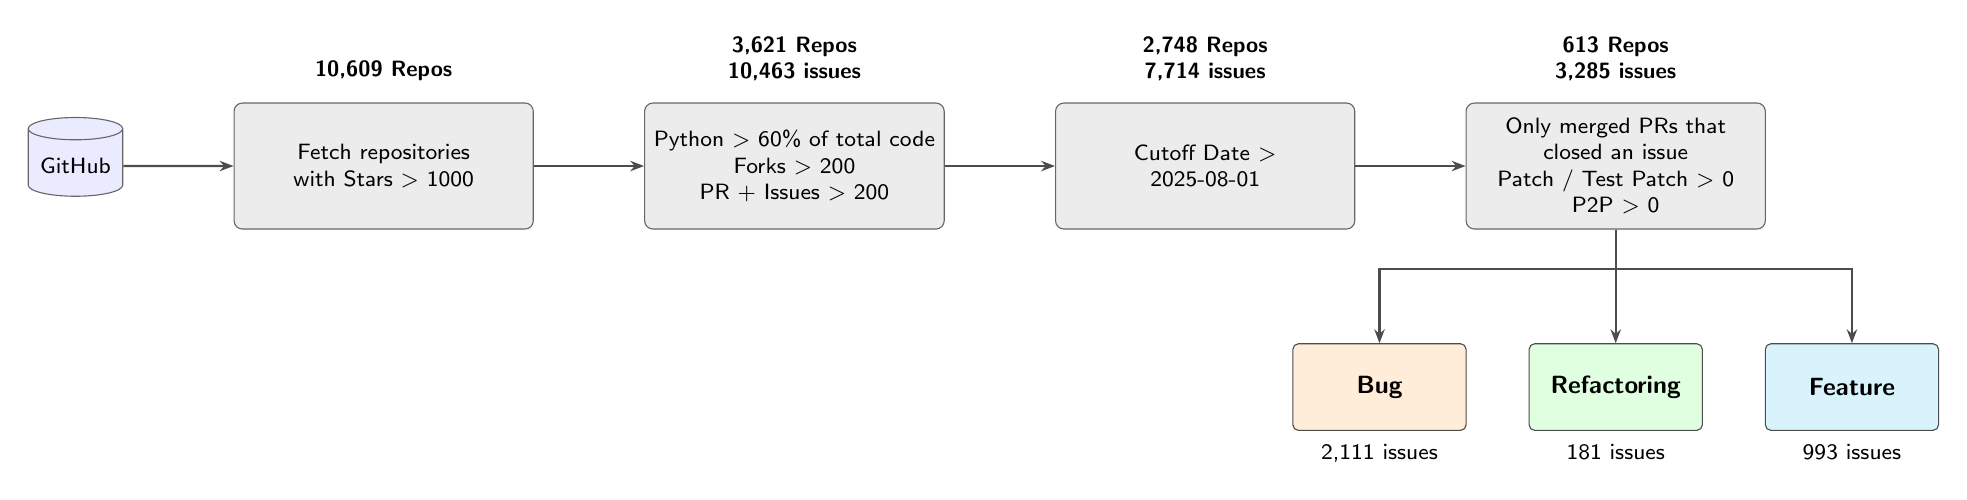
\begin{tikzpicture}[
    node distance=0.6cm and 1.2cm,
    box/.style={rectangle, draw=black!60, fill=gray!15, rounded corners=3pt,
                minimum height=1.6cm, minimum width=3.8cm, align=center,
                font=\footnotesize},
    countbox/.style={font=\footnotesize\bfseries, align=center, above=0.15cm},
    arrow/.style={-{Stealth[length=5pt]}, thick, draw=black!70},
    db/.style={cylinder, draw=black!60, fill=blue!8, shape border rotate=90,
               aspect=0.25, minimum height=1cm, minimum width=1.2cm,
               font=\footnotesize, align=center},
    catbox/.style={rectangle, draw=black!70, fill=blue!10, rounded corners=2pt,
                   minimum height=1.1cm, minimum width=2.2cm, align=center,
                   font=\small\bfseries},
]

% GitHub source
\node[db] (github) {GitHub};

% Stage 1: Fetch repos
\node[box, right=1.4cm of github] (s1) {Fetch repositories\\with Stars $>$ 1000};
\node[countbox] at (s1.north) {10,609 Repos};

% Stage 2: Language/activity filter
\node[box, right=1.4cm of s1] (s2) {Python $>$ 60\% of total code\\Forks $>$ 200\\PR + Issues $>$ 200};
\node[countbox] at (s2.north) {3,621 Repos\\10,463 issues};

% Stage 3: Date filter
\node[box, right=1.4cm of s2] (s3) {Cutoff Date $>$\\2025-08-01};
\node[countbox] at (s3.north) {2,748 Repos\\7,714 issues};

% Stage 4: Merge/patch filter
\node[box, right=1.4cm of s3] (s4) {Only merged PRs that\\closed an issue\\Patch / Test Patch $>$ 0\\P2P $>$ 0};
\node[countbox] at (s4.north) {613 Repos\\3,285 issues};

% Arrows
\draw[arrow] (github) -- (s1);
\draw[arrow] (s1) -- (s2);
\draw[arrow] (s2) -- (s3);
\draw[arrow] (s3) -- (s4);

% Classification branches
\node[catbox, fill=orange!15] (bug) at ($(s4.south) + (-3.0, -2.0)$) {Bug};
\node[below=0.05cm of bug, font=\footnotesize] {2,111 issues};

\node[catbox, fill=green!12] (refactoring) at ($(s4.south) + (0, -2.0)$) {Refactoring};
\node[below=0.05cm of refactoring, font=\footnotesize] {181 issues};

\node[catbox, fill=cyan!15] (feature) at ($(s4.south) + (3.0, -2.0)$) {Feature};
\node[below=0.05cm of feature, font=\footnotesize] {993 issues};

% Branch arrows from s4 to categories
\draw[arrow] (s4.south) -- ++(0, -0.5) -| (bug.north);
\draw[arrow] (s4.south) -- ++(0, -0.5) -| (refactoring.north);
\draw[arrow] (s4.south) -- ++(0, -0.5) -| (feature.north);

\end{tikzpicture}
\end{document}
